\begin{quote}
Review

Author(s): Eric Geoffroy Review by: Eric Geoffroy

Source: \emph{Studia Islamica,} No. 91 (2000), pp. 214-215 Published by:
\href{http://www.jstor.org/action/showPublisher?publisherCode=mal}{Maisonneuve
\& Larose}

Stable URL: \url{http://www.jstor.org/stable/1596284} Accessed:
09-08-2015 13:31 UTC

Your use of the JSTOR archive indicates your acceptance of the Terms \&
Conditions of Use, available at
\href{http://www.jstor.org/page/info/about/policies/terms.jsp}{\underline{http://www.jstor.org/page/}}
\href{http://www.jstor.org/page/info/about/policies/terms.jsp}{\underline{info/about/policies/terms.jsp}}

JSTOR is a not-for-profit service that helps scholars, researchers, and
students discover, use, and build upon a wide range of content in a
trusted digital archive. We use information technology and tools to
increase productivity and facilitate new forms of scholarship. For more
information about JSTOR, please contact
\href{mailto:support@jstor.org}{support@jstor.org.}

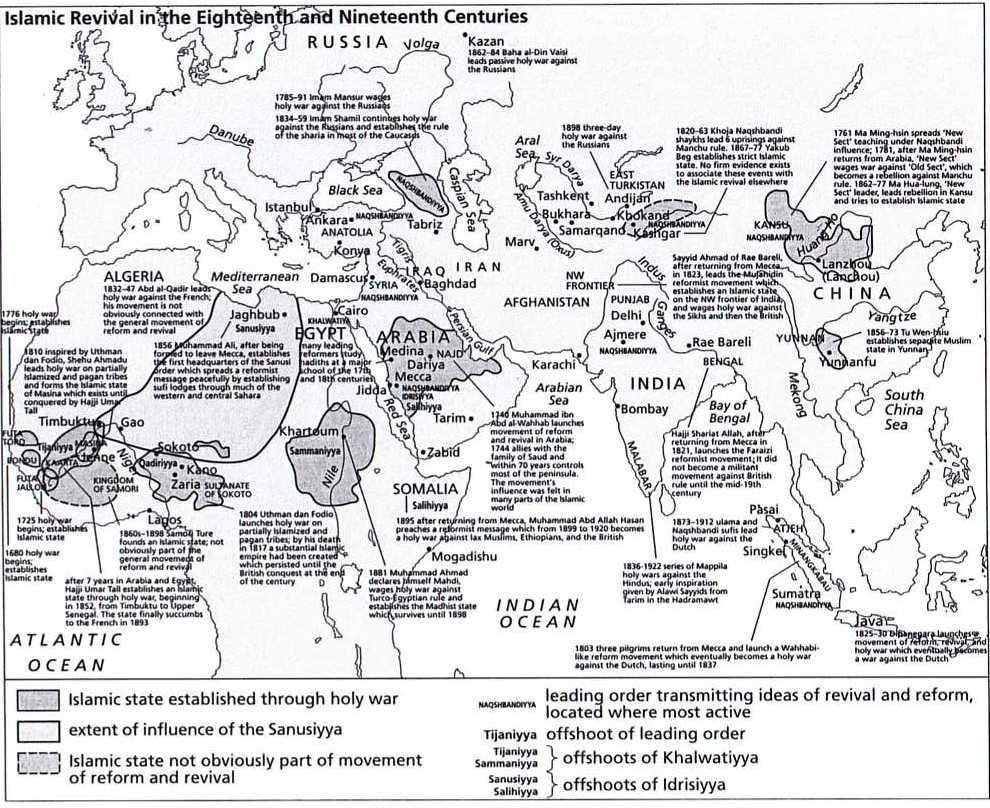
\includegraphics[width=0.48958in,height=0.625in]{media/image1.jpeg}\emph{Maisonneuve
\& Larose} is collaborating with JSTOR to digitize, preserve and extend
access to \emph{Studia Islamica.}

\href{http://www.jstor.org/}{\underline{http://www.jstor.org}}
\end{quote}

\hypertarget{this-content-downloaded-from-41.178.157.149-on-sun-09-aug-2015-133114-utc-all-use-subject-to-jstor-terms-and-conditions}{%
\subsection{\texorpdfstring{This content downloaded from 41.178.157.149
on Sun, 09 Aug 2015 13:31:14 UTC All use subject to
\href{http://www.jstor.org/page/info/about/policies/terms.jsp}{\underline{JSTOR
Terms and
Conditions}}}{This content downloaded from 41.178.157.149 on Sun, 09 Aug 2015 13:31:14 UTC All use subject to JSTOR Terms and Conditions}}\label{this-content-downloaded-from-41.178.157.149-on-sun-09-aug-2015-133114-utc-all-use-subject-to-jstor-terms-and-conditions}}

\begin{quote}
BOOKREVIEW

Frederick De J0NG et Bernd RADTKE (sous la dir.), \emph{lslamic
Mysticism Contested} - \emph{Thir­ teen Centuries of Controversies and
Polemics,} Leiden, Brill, 1999, 829 p.

« Entre les spirituels musulmans et \emph{lesfuqaha'} il y a une lutte
incessante et des com­ bats qui ne prendront fin que devant le Seigneur
de gloire, au Grand jour ». Le soufi damascène 'Afif al-Din al-Tilimsâni
(m. 690/1291) évoquait en ces termes pessimistes la divergence de
perspective existant entre les exotéristes et les ésotéristes de
l'islam. Les

« docteurs de la Loi » n'ont certes pas été les seuls antagonistes des
soufis ; un autre axe essentiel de conflits a une nature directement
politique, puisqu'il concerne les rapports entre autorité spirituelle et
pouvoir temporel. Par ailleurs, les milieux soufis ne constituent pas un
monde homogène, et encore moins monolithique ; différentes options -
spiri­ tuelles, mais aussi sociales ou politiques - s'y dessinent,
parfois contradictoires. Les cri­ tiques et polémiques suscitées au sein
du soufisme, bien souvent sur fond de rivalité inter­ \emph{farîqa,}
déterminent ainsi une troisième ligne de fracture.

L'ouvrage collectif édité ici par F. De Jong et B. Radtke aborde ces
thèmes tour à tour, au fil des trente-trois contributions qui le
composent. Il s'agit des actes d'un colloque inter­ national intitulé «
Sufism and its Opponents », lequel se tint à Utrecht (Pays Bas), du l"
au 6 mai 1995. En introduction, les éditeurs justifient leur projet par
le fait qu'il n'exis­ tait pas jusqu'alors d'étude comparative sur la
question; ils soulignent également que la polémique anti-soufie est
toujours d'actualité et qu'elle se manifeste, par exemple, dans la
violence exercée par divers groupes « fondamentalistes » à l'égard des
soufis contempo­ rains (p. 1-2).

À l'islamologue allemand J. van Ess est confié le soin de mener une«
réflexion» intro­ ductive générale sur« le soufisme et ses opposants».
Au cours de ce survol, forcément rapide, van Ess met le doigt sur
quelques épicentres majeurs du conflit soufis / non-sou­ fis, qui
forment autant de points développés par les autres intervenants (le
soufisme dans ses rapports avec : le hanbalisme, le mu 'tazilisme, le
chiisme, Ibn Taymiyya, le réfor­ misme). Suit la seule partie thématique
de l'ouvrage, un peu hétéroclite, où sont traités cer­ tains de ces
points : les origines du contentieux dans le soufisme primitif (article
très sub­ tantiel, sur le plan doctrinal, de G. Bowering, mais qui
n'aborde que partiellement le sujet), puis les attitudes mu 'tazilite,
zaydite, wahhabite, la question d'lbn 'Arabi, la situation par­
ticulière du « néo-soufisme » (xvm' - XIX' s.).

Les six autres parties, quant à elles, adoptent un découpage
géographique : Maghreb et Moyen-Orient, Afrique, Inde, etc. Cet
agencement a l'avantage de couvrir la quasi-tota­ lité du monde
musulman, mais du coup il privilégie la périphérie de ce dernier. Le
Moyen Orient se trouve ainsi sous-représenté (comme le reconnaissent les
éditeurs dans la post­ face, p. 759), alors qu'il constitue le foyer
premier et central des polémiques contre le sou­ fisme. Ce découpage
géographique se fait au détriment de la dimension historique du dos­
sier, car la grande majorité des communications présentées dans ces six
parties concerne les périodes moderne et contemporaine. Or, la
rhétorique anti-soufie se met en place très tôt, et les éditeurs
eux-mêmes en soulignent la « nature répétitive » (p. 760). On cherche
toujours appui, en islam, sur des autorités plus anciennes. Si la
position de l'école mu 'tazi­ lite d'un côté et d'Ibn l:fanbal de
l'autre a remarquablement été étudiée par F. Sobieroj (pp. 68-92), on
aimerait en savoir plus sur certains propos attribués à l'imam Malik ou
à l'imam al-Sâfi'i. La critique d'lbn al-Gawzi, à laquelle répondront
maints soufis posté­ rieurs, a été à peine mentionnée. L'art. de T.E.
Homerin, sur cette Égypte mamelouke où le soufisme tient une place si
prédominante, est trop superficiel (par ex. il ne cerne
\end{quote}

\hypertarget{section}{%
\section{214}\label{section}}

\begin{quote}
REVUE DES LIVRES

pas assez l'aspect « soufi » d'Ibn Taymiyya, n'évoque pas le modèle du «
savant-soufi »

très valorisé durant cette période ; l'auteur n'a pas su non plus
analyser le clivage

\emph{!Jiinqiih/ziiwiya).} La contribution fort documentée de M.
Chodkiewicz sur « le procès posthume d'Ibn 'Arabi » montre bien, quant à
elle, que les diatribes menées contre l'au­ teur des \emph{Fu\$û\$
al-/:likam} n'évoluent quasiment plus à partir du xv' siècle.

Diverses remarques pourraient être faites ici ou là. Par exemple, p. 284
: le divorce entre soufisme et chiisme safavide s'est produit non à la
fin du xvr siècle, mais dès la prise du pouvoir par Siih Ismii'il, qui a
banni le terme \emph{ta\$awwuf} pour le remplacer par \emph{'i,fàn;} ou
encore pp.611-612, où la doctrine de la \emph{wa/:ldat al-wugüd} est
présentée comme un élément d'opposition populaire au régime ottoman,
alors que celui-ci, on le sait, a pris fait et cause dès ses origines
pour Ibn 'Arabi et son œuvre. Mais, plus fonfamentalement, il manque
toute une dimension dans l'analyse du sujet : celle des attaques que les
soufis ont à leur tour adressées aux exotéristes de l'islam. Le
sous-titre de l'ouvrage laisse pour­ tant bien entendre que les «
controverses et polémiques » venaient de part et d'autre. Or, hormis la
contribution d'A. Buehler sur « la réponse naqshbandi aux censeurs du
soufisme », il aura été peu dit que les soufis contestaient les
capacités spirituelles mais aussi intellec­ tuelles des \emph{fuqahii}
', et qu'ils dénonçaient la corruption des notables religieux
(l'opposition aux pouvoirs politiques a davantage été mise en exergue).
À ce titre, un article sur le duel que les soufis ont fait jouer aux
termes \emph{faqihlfaqir} aurait été bienvenu. De même, un auteur comme
Sii'riini (xv!"s.) aurait pu être étudié (notamment son ouvrage encore
inédit \emph{al-Agwiba al-marçiyya 'an a'imma al-fuqahii' wa l-
ûfiyya),} car son œuvre a servi de réfé­ rence à beaucoup de soufis
ayant croisé le fer avec \emph{lesfuqahii'.} La caution qu'ont appor­
tée des savants notoires de cette époque (Suyü!i, Ibn I:Iagar
al-Haytami...) en prenant le défense du soufisme dans le cadre de
\emph{lafatwii} méritait, elle aussi, d'être soulignée. Leur
revendication d'un \emph{igtihiid} proprement spirituel, fondé sur le «
dévoilement » \emph{(kas!),} marque une avancée décisive dans le rapport
de forces avec \emph{lesfuqahii'.}

Différents contributeurs ont fort judicieusement remarqué qu'il faut
être doté d'un grand sens de la nuance pour voir clair dans ces débats.
En effet, les polémiques et les conflits sont souvent \emph{internes au
soufisme} car, nous l'avons dit, diverses modalités, diverses tendances
se côtoient dans la sphère du \emph{ta awwuf} li y a toujours eu des
cheikhs « réformistes », prompts à stigmatiser tel ou tel comportement
d'autres mystiques, et chaque soufi a son « pseudo­ soufi ». Il y a des
soufis \emph{fuqahii',} et des soufis \emph{sala.fi} ; certains ont même
pu trouver un ter­ rain d'entente avec les wahhabites (voir p. 147,
757). Plusieurs mouvements dits soufis, à l'époque moderne ou
contemporaine, se distinguent à peine de ceux qui relèvent du « fon­
damentalisme » islamique (p. 759). Enfin, les éditeurs ont raison de
voir dans la pérennité et la vivacité des débats que soulève le soufisme
un indice à la fois de la vitalité et du plu­ ralisme de l'islam ; et de
rappeler le \emph{hadi!} bien connu : « Les différends au sein de ma
com­ munauté sont une miséricorde».

Les 760 pages de textes sont heureusement suivies d'index détaillés, qui
permettent

d'exploiter au mieux l'énorme masse d'informations prodiguée dans
l'ouvrage.
\end{quote}

Eric GEOFFROY

(Université Marc Bloch - Strasbourg II)

\hypertarget{section-1}{%
\section{215}\label{section-1}}
